%-------------------------------------------------------------------------------
%                                PREAMBLE
%-------------------------------------------------------------------------------
\documentclass[usenames,dvipsnames,svgnames,10pt,aspectratio=169]{beamer}
\usefonttheme{professionalfonts}

% This theme uses TIKZ: compile twice with PDFLaTeX or LuaLaTeX.
%
%  Options:
%  - [clean]:    clean slides, i.e. logos and footbar are removed
%  - [kth]:      footbar style inspierd to the official KTH template
%  - [nicewave]: a different style of wave is used (not approved by FLOW)
%
\usetheme{flow}

\usepackage{hyperref,graphicx,lmodern}
\usepackage[utf8]{inputenc}
\usepackage{media9}
\usepackage{xcolor}
\usepackage{stmaryrd}
\usepackage{nicefrac}
\usepackage{multimedia}
\usepackage{multicol}
\usepackage{upgreek}
\usepackage[]{bm}
\usepackage[]{url}


\DeclareMathAlphabet{\mathcal}{OMS}{cmsy}{m}{n}
\DeclareMathAlphabet\mathbfcal{OMS}{cmsy}{b}{n}

\graphicspath{{imgs/}}
\setbeamertemplate{blocks}[rounded][shadow=true]

\DeclareMathOperator{\trace}{tr}

%-------------------------------------------------------------------------------
%                                TITLE PAGE
%-------------------------------------------------------------------------------
\title[Nonlinear Physics] % Short title used in footline
{
	Nonlinear physics, dynamical \\ systems and chaos theory
}

\author[J.-Ch.~Loiseau] % Presenting author in short form used in footline
{
	Jean-Christophe Loiseau
}
% - Give the names in the same order as the appear in the paper.
% - Underline the presenting author.

\institute[unused]
{
	\url{jean-christophe.loiseau@ensam.eu} \\
	DynFluid, \\
	Arts et M\'etiers ParisTech, France
}
% Keep it simple, no one is interested in your street address.

% University logo(s)
\logot{
\includegraphics[width=.128\paperwidth]{DynFluid_logo}}  % Top logo
\logob{
\includegraphics[width=0.128\paperwidth]{ENSAM_logo}} % Bottom logo
% \logoc[{
\includegraphics[width=.128\paperwidth]{limsi}}]{
\includegraphics[width=.128\paperwidth]{limsi}} % Corner logo
%
% Cover image: \cvrimg{x position}{y position}{cover image}
\cvrimg{.77}{.8}{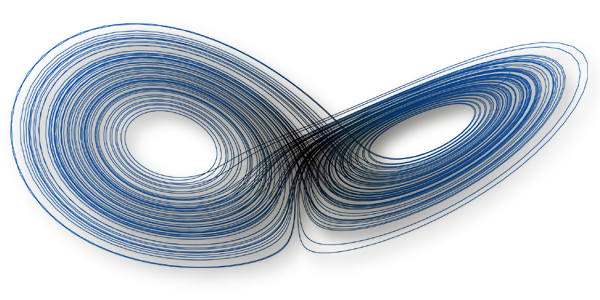
\includegraphics[width=.4\paperwidth]{cover.png}}

\date[unused]{ENSAM, Master 2, 2018--2019}

\begin{document}

\titleframe % Print the title as the first slide

%-------------------------------------------------------------------------------
%                           PRESENTATION SLIDES
%-------------------------------------------------------------------------------

\begin{frame}[t, c]{Overview from last time}{}
	Given the non-linear dynamical system
	\begin{equation}
		\dot{\mathbf{X}} = \mathbfcal{F}\left( \mathbf{X} \right),
		\notag
	\end{equation}
	we have seen in the previous lectures how to :
	\begin{itemize}
		\item[$\hookrightarrow$] Compute fixed points $\mathbf{X}^*$ of the system, i.e.\ solutions to
		$$\mathbfcal{F}\left( \mathbf{X} \right) = 0.$$

		\item[$\hookrightarrow$] Derive the linearized the equations governing the dynamics of a perturbation $\mathbf{x}$ :
		$$\dot{\mathbf{x}} = \mathbfcal{A} \mathbf{x}.$$

		\item[$\hookrightarrow$] Characterize the linear stability of the fixed point $\mathbf{X}^*$ based on the eigenspectrum of $\mathbfcal{A}$.
	\end{itemize}

	\vspace{1cm}
\end{frame}

\begin{frame}[t, c]{}{}
	\begin{block}{\centering \textbf{Question}}
		Let us now consider a parametrized dynamical system
		$$\dot{\mathbf{x}} = \mathbfcal{F}\left( \mathbf{x}, \mu \right).$$
		How do its fixed points evolve when varying the parameter $\mu$? Can we characterize this evolution and make predictions?
	\end{block}
\end{frame}

\begin{frame}[t, c]{}
	\centering
	\vspace{1cm}

	{\Large \textbf{Bifurcations of first-order systems}}

	\bigskip

	{\textgre{\textbf{Flows on the line (again)}}}

\end{frame}

\begin{frame}[t, c]{Bifurcations of first-order systems}{}
	\begin{itemize}
		\item Let us consider a first-order dynamical system
		$$\dot{x} = f(x, \mu),$$
		where $\mu$ is our \alert{\textbf{control parameter}}.

		\bigskip

		\item We have seen that such systems have relatively simple dynamics dictated by fixed points.

		\bigskip

		\item These fixed points may however change as a function of $\mu$.
		\begin{itemize}
			\item[$\hookrightarrow$] Qualitative variations of the dynamics are called \alert{\textbf{bifurcations}}.
			\item[$\hookrightarrow$] The values of $\mu$ at which these changes occurs are called \alert{\textbf{bifurcation points}}.
		\end{itemize}
	\end{itemize}

	\vspace{2cm}
\end{frame}

\begin{frame}[t, c]{Bifurcations of first-order systems}{}
	\begin{itemize}
		\item To facilitate discussions to come, the Taylor expansion of $f(x)$ (for a constant $\mu$) is given by
		$$f(x) \simeq a_0 + a_1 x + a_2 x^2 + a_3 x^3 + a_4 x^4 + a_5 x^5 + \cdots$$

		\medskip

		\item Depending on the coefficients $a_k$, different behaviors will be observed.
	\end{itemize}

	\vspace{1cm}
\end{frame}

\begin{frame}[t, c]{Saddle-node bifurcation}{First-order dynamical system}
	\begin{itemize}
		\item As a starting point, let us look at the system
		$$\dot{x} = \mu - x^2$$
		and plot its phase line for different values of $\mu$.
	\end{itemize}

	\vspace{1cm}
\end{frame}

\begin{frame}[t, c]{Saddle-node bifurcation}{Phase line}
	\centering
	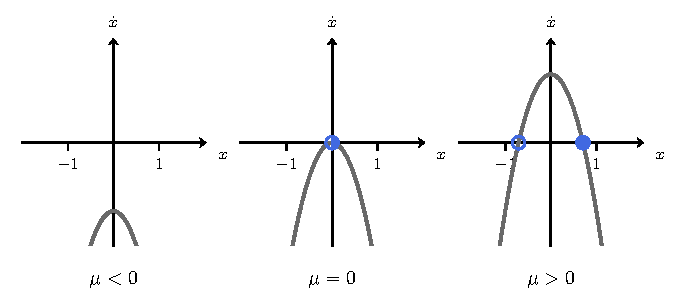
\includegraphics[width=.75\textwidth]{saddle_node_phase_line}

	Evolution of the phase line of the system for $\mu = \nicefrac{-1}{2}, 0$ and $\nicefrac{1}{2}$.

	\vspace{1cm}
\end{frame}

\begin{frame}[t, c]{Saddle-node bifurcation}{Fixed points and stability}
	\begin{itemize}
		\item Depending on the value of $\mu$, different behaviors are possible.
		\begin{itemize}
			\item[$\hookrightarrow$] For $\mu < 0$, the system admits no fixed points and $\lim \limits_{t \to \infty} x(t) = - \infty$.

			\item[$\hookrightarrow$] For $\mu = 0$, the system admits a single \alert{\textbf{meta-stable}} fixed point $x^* = 0$. For $x(0) > 0$, $\lim \limits_{t \to \infty} x(t) = 0$, otherwise, for $x(0) < 0$, $\lim \limits_{t \to \infty} x(t) = -\infty$.

			\item[$\hookrightarrow$] For $\mu > 0$, the system admits to fixed points $x^* = \pm \sqrt{\mu}$. One is linearly stable, while the other one is linearly unstable.
		\end{itemize}

		\bigskip

		\item As $\mu$ becomes positive, we observe a transition from the absence of fixed points to the creation of two of them, one stable and the other unstable. This is known as the \alert{\textbf{saddle node bifurcation}}.
	\end{itemize}

	\vspace{1cm}
\end{frame}

\begin{frame}[t, c]{Saddle-node bifurcation}{Bifurcation diagram}
	\centering
	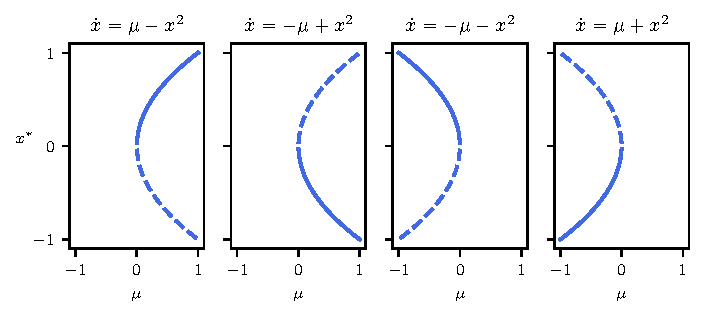
\includegraphics[width=.75\textwidth]{saddle_node_bifurcation_diagrams}

	Bifurcation diagrams for the different combinations of saddle-node bifurcations.
	\vspace{1cm}
\end{frame}

\begin{frame}[t, c]{Saddle-node bifurcation}{Example from real life}
	\begin{itemize}
		\item Let us consider a damped pendulum driven by a constant torque
		\begin{equation}
			m L^2 \displaystyle \frac{\mathrm{d}^2 \theta}{\mathrm{d}t^2} + b \frac{\mathrm{d} \theta}{\mathrm{d}t} + mgL \sin (\theta) = \Gamma.
			\notag
		\end{equation}

		\bigskip

		\item Introducing the time scale $t = T \tau$, one can write
		\begin{equation}
			\displaystyle \frac{L}{gT^2} \ddot{\theta} + \frac{b}{mgL T} \dot{\theta} + \sin(\theta) = \frac{\Gamma}{mgL}.
			\notag
		\end{equation}
	\end{itemize}

	\vspace{1cm}
\end{frame}

\begin{frame}[t, c]{Saddle-node bifurcation}{Example from real life}
	\begin{itemize}
		\item If $\nicefrac{b}{mgT} \gg \nicefrac{L}{gT^2}$, we can neglect $\ddot{\theta}$ and our equation becomes
		\begin{equation}
			\dot{\theta} = \gamma - \sin ( \theta ),
			\notag
		\end{equation}
		with $T = \nicefrac{b}{mgL}$ and $\gamma = \nicefrac{\Gamma}{mgL}$.

		\bigskip

		\item You can now easily show that the system experiences a saddle-node bifurcation at $\gamma = 1$.

		\bigskip

		\item Interpret your results from physical point of view!
	\end{itemize}

	\vspace{1cm}
\end{frame}

\begin{frame}[t, c]{Transcritical bifurcation}{First-order dynamical system}
	\begin{itemize}
		\item Let us now consider the following first-order dynamical system
		$$\dot{x} = \mu x - x^2$$
		and plot its phase line for different values of $\mu$.
	\end{itemize}

	\vspace{1cm}
\end{frame}

\begin{frame}[t, c]{Transcritical bifurcation}{Phase line}
	\centering
	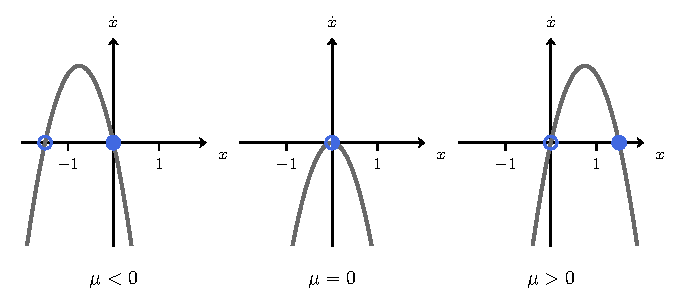
\includegraphics[width=.75\textwidth]{transcritical_phase_line}

	Evolution of the phase line of the system for $\mu = \nicefrac{-3}{2}, 0$ and $\nicefrac{3}{2}$.

	\vspace{1cm}
\end{frame}

\begin{frame}[t, c]{Transcritical bifurcation}{Fixed points and linear stability}
	\begin{itemize}
		\item The system admits two fixed points
		$$x_1^ * = 0 \text{ and } x_2^* = \mu.$$

		\item Depending on the sign of $\mu$, we have
		\begin{itemize}
			\item[$\hookrightarrow$] For $\mu < 0$, $x_1^*$ is linearly stable while $x_2^*$ is linearly unstable.
			\item[$\hookrightarrow$] For $\mu=0$, $x_1^* = x_2^*$ is meta-stable.
			\item[$\hookrightarrow$] For $\mu > 0$, $x_1^*$ is now linearly unstable, while $x_2^*$ has become linearly stable.
		\end{itemize}

		\medskip

		\item As $\mu$ becomes positive, the two fixed points have exchanged their stability. This is known as the \alert{\textbf{transcritical bifurcation}}.
	\end{itemize}

	\vspace{1cm}
\end{frame}

\begin{frame}[t, c]{Transcritical bifurcation}{Bifurcation diagram}
	\centering
	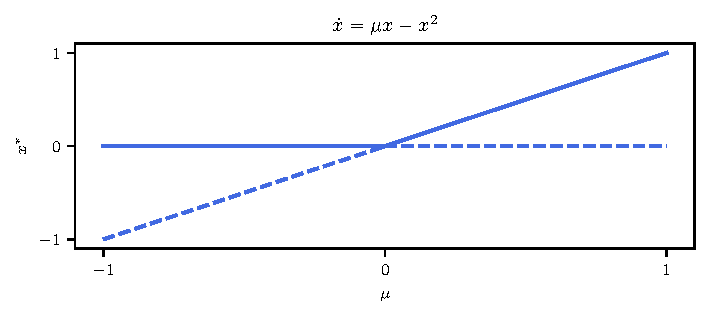
\includegraphics[width=.75\textwidth]{transcritical_bifurcation_diagram}

	Bifurcation diagram of the transcritical bifurcation.
	\vspace{1cm}
\end{frame}

% \begin{frame}[t, c]{Transcritical bifurcation}{Example from real life}
%
% \end{frame}

\begin{frame}[t, c]{Supercritical pitchfork bifurcation}{First-order dynamical system}
	\begin{itemize}
		\item Let us consider the following system
		$$\dot{x} = \mu x - x^3$$
		and plot its phase line for different values of $\mu$.
	\end{itemize}

	\vspace{1cm}
\end{frame}

\begin{frame}[t, c]{Supercritical pitchfork bifurcation}{Phase line}
	\centering
	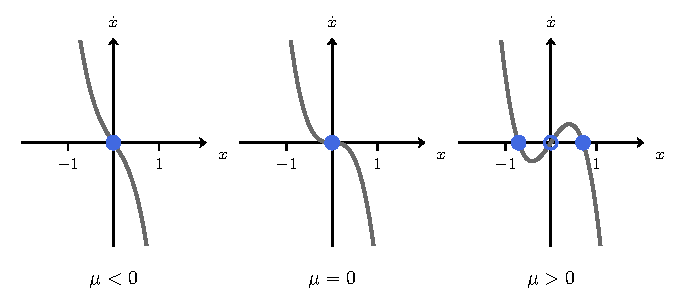
\includegraphics[width=.75\textwidth]{supercritical_pitchfork_phase_line}

	Evolution of the phase line of the system for $\mu = \nicefrac{-1}{2}, 0$ and $\nicefrac{1}{2}$.

	\vspace{1cm}
\end{frame}

\begin{frame}[t, c]{Supercritical pitchfork bifurcation}{Fixed points and linear stability}
	\begin{itemize}
		\item Depending on the value of $\mu$, different behaviors are possible.
		\begin{itemize}
			\item[$\hookrightarrow$] For $\mu<0$, the system admits a single linearly stable fixed point $x^* = 0$.
			\item[$\hookrightarrow$] For $\mu = 0$, the fixed point $x^*=0$ is marginal from a linear point of view, yet still nonlinearly stable.
			\item[$\hookrightarrow$] For $\mu > 0$, the system now admits three fixed points. $x_1^*=0$ is now linearly unstable, while $x^*_{2, 3} = \pm \sqrt{\mu}$ are linearly stable.
		\end{itemize}

		\medskip

		\item As $\mu$ becomes positive, we observe that the origin becomes linearly unstable and two additional stable fixed points are created. This is known as the \alert{\textbf{supercritical pitchfork bifurcation}}.
	\end{itemize}

	\vspace{1cm}
\end{frame}

\begin{frame}[t, c]{Supercritical pitchfork bifurcation}{Bifurcation diagram}
	\centering
	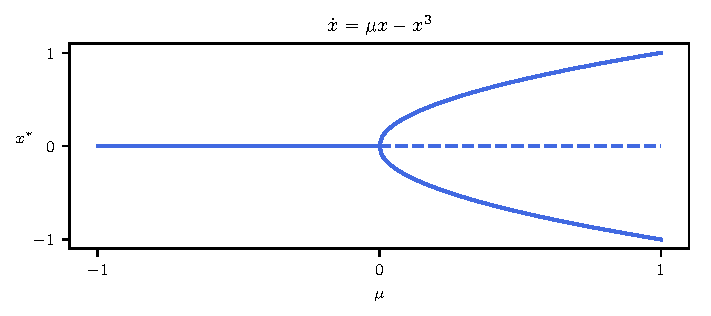
\includegraphics[width=.75\textwidth]{supercritical_pitchfork_bifurcation_diagram}

	Bifurcation of the supercritical pitchfork.

	\vspace{1cm}
\end{frame}


\begin{frame}[t, c]{Subcritical pitchfork bifurcation}{First-order dynamical system}
	\begin{itemize}
		\item Let us consider the following system
		$$\dot{x} = \mu x + x^3$$
		and plot its phase line for different values of $\mu$.
	\end{itemize}

	\vspace{1cm}
\end{frame}

\begin{frame}[t, c]{Subcritical pitchfork bifurcation}{Phase line}
	\centering
	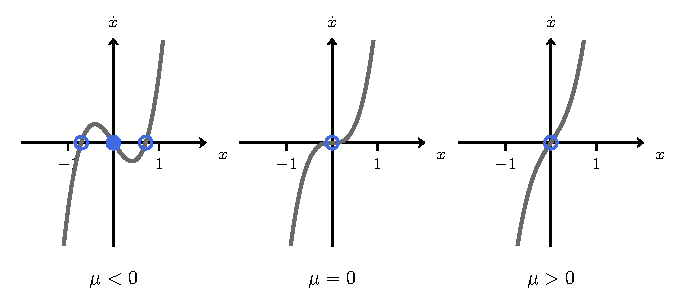
\includegraphics[width=.75\textwidth]{subcritical_pitchfork_phase_line}

	Evolution of the phase line of the system for $\mu = \nicefrac{-1}{2}, 0$ and $\nicefrac{1}{2}$.

	\vspace{1cm}
\end{frame}

\begin{frame}[t, c]{Subcritical pitchfork bifurcation}{Fixed points and linear stability}
	\begin{itemize}
		\item Depending on the value of $\mu$, different behaviors are possible.
		\begin{itemize}
			\item[$\hookrightarrow$] For $\mu < 0$, the system admits three fixed points. $x_1^*=0$ is linearly stable, while $x^*_{2, 3} = \pm \sqrt{-\mu}$ are linearly unstable.
			\item[$\hookrightarrow$] For $\mu = 0$, the fixed point $x^*=0$ is marginal from a linear point of view, but nonlinearly unstable.
			\item[$\hookrightarrow$] For $\mu<0$, the system now admits a single linearly unstable fixed point $x^* = 0$.
		\end{itemize}

		\medskip

		\item As $\mu$ becomes positive, we observe that the origin becomes linearly unstable and the other two unstable fixed points are destroyed. This is known as the \alert{\textbf{subcritical pitchfork bifurcation}}.
	\end{itemize}

	\vspace{1cm}
\end{frame}

\begin{frame}[t, c]{Subcritical pitchfork bifurcation}{Bifurcation diagram}
	\centering
	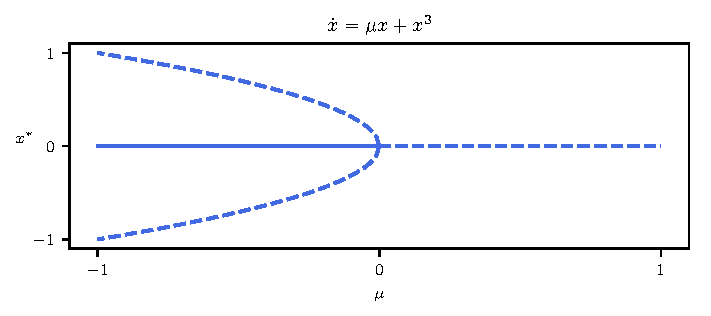
\includegraphics[width=.75\textwidth]{subcritical_pitchfork_bifurcation_diagram}

	Bifurcation of the subcritical pitchfork.

	\vspace{1cm}

\end{frame}

% \begin{frame}[t, c]{Pitchfork bifurcation}{Example from real life}
%
% \end{frame}

\begin{frame}[t, c]{Bifurcations of first-order systems}{Summary}
	\centering
	\begin{tabular}{l|cccccc}
		~ & $f$ & $f_x$ & $f_{\mu}$ & $f_{xx}$ & $f_{x \mu}$ & $f_{xxx}$ \\
		\hline
		Fixed point & $0$ \\
		Bifurcation  & $0$ & $0$ & $\neq 0$ \\
		Saddle-node & $0$ & $0$ & $\neq 0$ & $\neq 0$\\
		Transcritical & $0$ & $0$ & $0$ & $\neq 0$ & $\neq 0$\\
		Pitchfork & $0$ & $0$ & $0$ & $0$ & $\neq 0$ & $\neq 0$\\
	\end{tabular}

	\vspace{1cm}
\end{frame}

\begin{frame}[t, c]{Exercise}
	\begin{itemize}
		\item Consider the following dynamical system
		$$\dot{x} = \mu x + x^3 - 0.25 x^5$$
		and study its different fixed points and bifurcations.
	\end{itemize}

	\vspace{1cm}
\end{frame}

\begin{frame}[t, c]{}
	\centering
	\vspace{1cm}

	{\Large \textbf{Bifurcations of second-order systems}}

	\bigskip

	{\textgre{\textbf{Creation of limit cycles}}}

\end{frame}

\begin{frame}[t, c]{Bifurcations of second-order systems}{}
	\begin{itemize}
		\item Let us now consider a second-order dynamical system given by
		\begin{equation}
			\begin{aligned}
				\dot{x} & = f(x, y, \mu) \\
				\dot{y} & = g(x, y, \mu).
			\end{aligned}
			\notag
		\end{equation}

		\item As seen in the previous lectures, such systems have dynamics much richer that those of first-order systems.

		\medskip

		\item How do they evolve as the control parameter $\mu$ changes?
		\begin{itemize}
			\item[$\hookrightarrow$] Note that all bifurcations seen so far also apply to fixed points of second-order dynamical systems.
		\end{itemize}
	\end{itemize}

	\vspace{1cm}
\end{frame}

\begin{frame}[t, c]{Saddle-node bifurcation revisited}{The reason it is called saddle-node}
	\begin{itemize}
		\item Consider the following system
		\begin{equation}
			\begin{aligned}
				\dot{x} & = \mu - x^2 \\
				\dot{y} & = - y
			\end{aligned}
			\notag
		\end{equation}
		and draw qualitatively its phase space for $\mu < 0$, $\mu = 0$ and $\mu > 0$.
	\end{itemize}

	\vspace{1cm}
\end{frame}

\begin{frame}[t, c]{Saddle-node bifurcation revisited}{The reason it is called saddle-node}
	\centering
	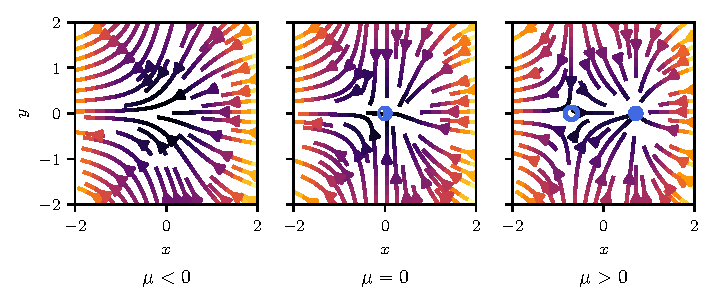
\includegraphics[width=.75\textwidth]{saddle_node_phase_plane}

	Phase plane of the system considered for varying $\mu$.
\end{frame}

\begin{frame}[t, c]{Hopf bifurcation}{Creation of limit cycles}
	\begin{itemize}
		\item Let us consider the following system
		\begin{equation}
			\begin{aligned}
				\dot{x} & = \mu x - \omega y - (x^2 + y^2)x \\
				\dot{y} & = \omega x + \mu y - (x^2 + y^2)y.
			\end{aligned}
			\notag
		\end{equation}

		\medskip

		\item It admits a single fixed point given by
		$$(x^*, y^*) = (0, 0).$$
	\end{itemize}

	\vspace{1cm}
\end{frame}

\begin{frame}[t, c]{Hopf bifurcation}{Exercise}
	\begin{enumerate}
		\item Study the linear stability of the fixed point as $\mu$ varies.
		\item Introducing the complex variable $z = x + iy$, show that the equation for $z$ reads
		$$\dot{z} = (\mu + i\omega)z - \vert z \vert^2z.$$
		\item From this complex equation, determine the first-order system that governs the amplitude of oscillation $r = \sqrt{x^2 + y^2}$.
		\item Study the properties of this equation an determine what type of bifurcation does the first-order system $\dot{r} = f(r, \mu)$ experiences.
		\item Sketch the evolution of the phase plane of our original system as $\mu$ varies and conclude.
	\end{enumerate}

	\vspace{1cm}
\end{frame}

\begin{frame}[t, c]{Hopf bifurcation}{Phase plane}
	\centering
	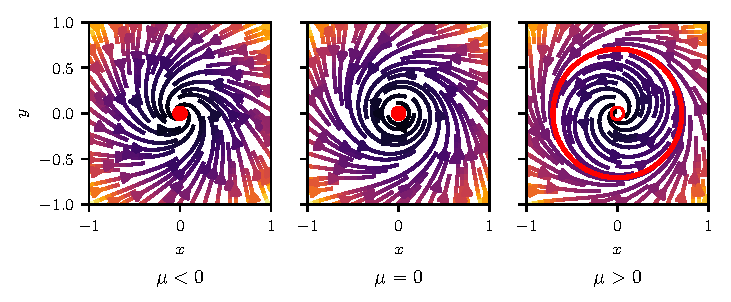
\includegraphics[width=.75\textwidth]{supercritical_hopf_bifurcation_phase_plane}

	Evolution of the phase plane of the system as a function of $\mu$ for the \alert{\textbf{supercritical Hopf bifurcation}}.

	\vspace{1cm}
\end{frame}


\begin{frame}[t, c]{Hopf bifurcation}{Phase plane}
	\centering
	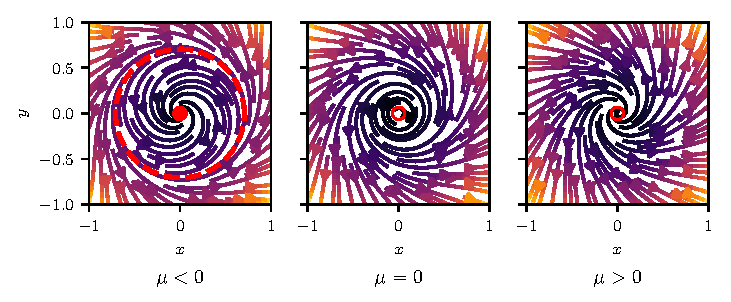
\includegraphics[width=.75\textwidth]{subcritical_hopf_bifurcation_phase_plane}

	Evolution of the phase plane of the system as a function of $\mu$ for the \alert{\textbf{subcritical Hopf bifurcation}}.

	\vspace{1cm}
\end{frame}

\begin{frame}[t, c]{Hopf bifurcation}{Normal form}
	\begin{itemize}
		\item The \alert{\textbf{normal form}} of the Hopf bifurcation (in polar coordinates) reads
		\begin{equation}
			\begin{aligned}
				\dot{r} & = \mu r \pm r^3 \\
				\dot{\theta} & = \omega,
			\end{aligned}
			\notag
		\end{equation}
		where $r$ is the amplitude of oscillator and $\theta$ its phase.
	\end{itemize}

	\vspace{1cm}
\end{frame}

\begin{frame}[t, c]{Hopf bifurcation}{Example from real life}
	\begin{minipage}{0.48\textwidth}
		\begin{itemize}
			\item The dynamics of the flow are governed by the Navier-Stokes equations
			\begin{equation}
				\begin{aligned}
					\displaystyle \frac{\partial {\bm u}}{\partial t} + ({\bm u} \cdot \nabla ) {\bm u} & = - \nabla p + \frac{1}{Re}\nabla^2 {\bm u}\\
					\nabla \cdot {\bm u} & = 0.
				\end{aligned}
				\notag
			\end{equation}

			\item These are partial differential equations having only a quadratic nonlinearity.

		\end{itemize}
	\end{minipage}%
	\hfill
	\begin{minipage}{0.48\textwidth}
		\begin{center}
			\movie[width=\textwidth, autostart, loop]{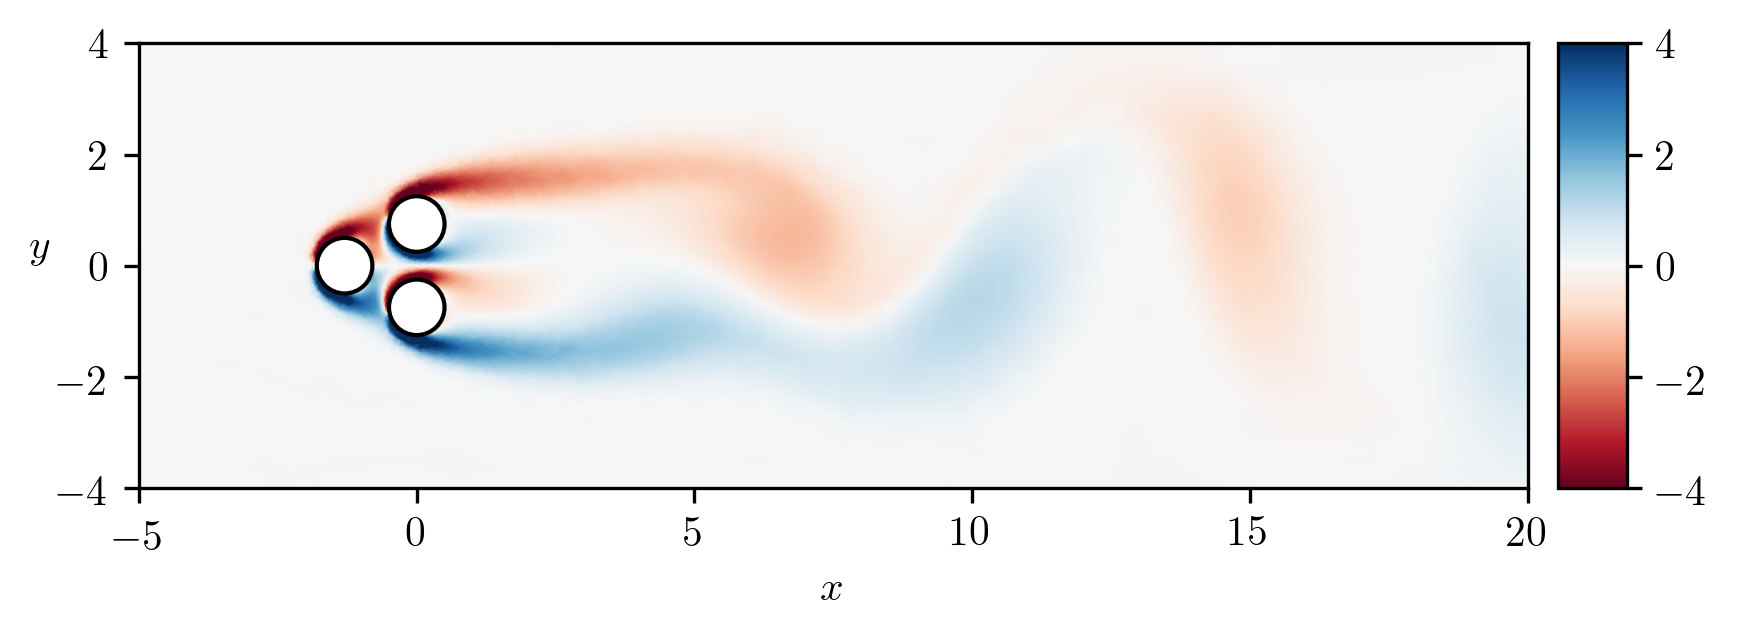
\includegraphics[width=\textwidth]{figure_100}}{imgs/out.mp4}
		\end{center}

		{\small Evolution of the vorticity field for the fluidic pinball at $Re=60$.}
	\end{minipage}

	\vspace{1cm}
\end{frame}

\begin{frame}[t, c]{Hopf bifurcation}{Example from real life}
	\begin{block}{\centering \textbf{Question}}
		\centering
		How come a system with quadratic nonlinearities exhibit a Hopf bifurcation whose normal form involve cubic ones?
	\end{block}

	\vspace{1cm}
\end{frame}

\begin{frame}[t, c]{Hopf bifurcation}{Example from real life}
	\begin{minipage}{.6\textwidth}
		These dynamics can be modeled by the following generalized mean-field model
			\begin{equation}
				\begin{aligned}
					\dot{x} & = \sigma x - y - xz \\
					\dot{y} & = x + \sigma y  - yz \\
					\dot{z} & = - \lambda( z - x^2 - y^2 ).
				\end{aligned}
				\notag
			\end{equation}
		where $x$ and $y$ capture the vortex shedding and $z$ describes the \emph{mean flow distortion}.
	\end{minipage}%
	\hfill
	\begin{minipage}{.28\textwidth}
		\centering
		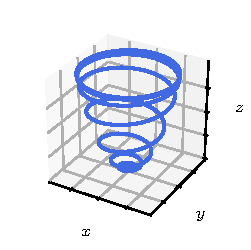
\includegraphics[width=.95\textwidth]{generalized_mean_field_model}

		{\small Trajectory given by the generalized mean field model.}
	\end{minipage}

	\vspace{1cm}
\end{frame}

\begin{frame}[t, c]{Hopf bifurcation}{Example from real life}
	\begin{minipage}{.6\textwidth}
		\begin{itemize}
			\item Let us compute the two-dimensional unstable manifold. For that purpose, assume
			\begin{equation}
				\begin{aligned}
					z & = h(x, y) \\
					~ & = a x^2 + b xy + c y^2.
				\end{aligned}
				\notag
			\end{equation}

			\bigskip

			\item After some calculations, we finally get
			$$z = \displaystyle \frac{1}{2\sigma + 1} \left( x^2 + y^2 \right).$$
			\begin{itemize}
				\item[$\hookrightarrow$] If $\lambda \gg \sigma$, the system rapidly evolves onto this two-dimensional paraboloid manifold.
			\end{itemize}
		\end{itemize}
	\end{minipage}%
	\hfill
	\begin{minipage}{.28\textwidth}
		\centering
		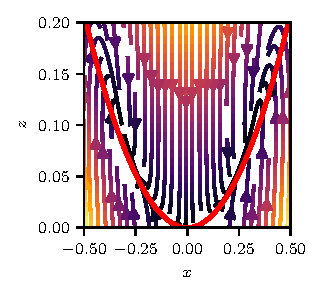
\includegraphics[width=.95\textwidth]{generalized_mean_field_model_manifold}

		{\small Slice in the $y=0$ plane of the phase space.}
	\end{minipage}

	\vspace{1cm}
\end{frame}

\begin{frame}[t, c]{Hopf bifurcation}{Example from real life}
	\begin{minipage}{.6\textwidth}
		\begin{itemize}
			\item Our dynamical system finally reduces to
			\begin{equation}
				\begin{aligned}
					\dot{x} & = \sigma x - y - \alpha (x^2 + y^2)x \\
					\dot{y} & = x + \sigma y - \alpha (x^2 - y^2)y.
				\end{aligned}
				\notag
			\end{equation}

			\medskip

			\item Introducing $A = x + iy$, we finally arrive to the normal form of the supercritical Hopf bifurcation
			$$\dot{A} = (\sigma + i)A - \alpha \vert A \vert^2 A.$$

			\medskip

			\item Though our system has only quadratic nonlinearities, dynamics on the manifold mimic cubic ones.
		\end{itemize}
	\end{minipage}%
	\hfill
	\begin{minipage}{.28\textwidth}
		\centering
		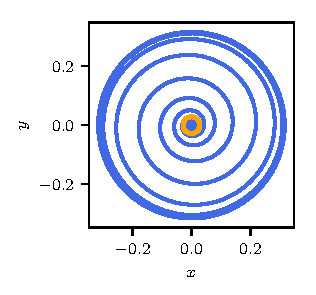
\includegraphics[width=.95\textwidth]{generalized_mean_field_model_2D}

		{\small Trajectory of the system on the 2D manifold.}
	\end{minipage}

	\vspace{1cm}
\end{frame}

\begin{frame}[t, c]{}
	\centering
	\vspace{1cm}

	{\Large \textbf{Stability of bifurcations}}

	\bigskip

	{\textgre{\textbf{Perturbing the very structure of the model}}}

\end{frame}

\begin{frame}[t, c]{Unperturbed normal forms}{What we have seen so far.}
	\centering
	\begin{itemize}
		\item So far, we have seen the following normal forms:
		\begin{itemize}
			\item[$\hookrightarrow$] Saddle-node :
			$$\dot{x} = \mu - x^2$$

			\item[$\hookrightarrow$] Transcritic :
			$$\dot{x} = \mu x- x^2$$

			\item[$\hookrightarrow$] Supercritical pitchfork :
			$$\dot{x} = \mu x - x^3$$

			\item[$\hookrightarrow$] Subcritical pitchfork :
			$$\dot{x} = \mu x + x^3$$

			\item[$\hookrightarrow$] Supercritical Hopf :
			\begin{equation}
				\begin{aligned}
					\dot{x} & = \mu x - \omega y + \left(x^2 + y^2 \right) \left(\alpha x - \beta y \right) \\
					\dot{y} & = \omega x + \mu y + \left(x^2 + y^2 \right) \left(\beta x + \alpha y \right).
				\end{aligned}
				\notag
			\end{equation}
		\end{itemize}
	\end{itemize}

	\vspace{1cm}
\end{frame}

\begin{frame}[t, c]{}{}

	\begin{block}{\centering \textbf{Question}}
		\centering
		What if we now perturb the very structure of the model (i.e.\ add an $\epsilon$ term)?
	\end{block}

	\vspace{-1cm}
\end{frame}


\begin{frame}[t, c]{}{}

	\begin{block}{\centering \textbf{Answer}}
		\centering
		This is your very first homework! It is due for early January.
	\end{block}

	\bigskip

	\begin{itemize}
		\item For each normal form, study the cases
			\begin{multicols}{3}
				\centering
				\item[$\hookrightarrow$] $\epsilon < 0$,
				\item[$\hookrightarrow$] $\epsilon = 0$,
				\item[$\hookrightarrow$] $\epsilon > 0$.
			\end{multicols}

		\item Which type of bifurcations are \emph{structurally} stable and which are not?
	\end{itemize}

	\vspace{-1cm}
\end{frame}

\end{document}
